\section{Einleitung}
\begin{frame}
	\frametitle{Einleitung}
	
	\begin{figure}
	   	\centering
	   	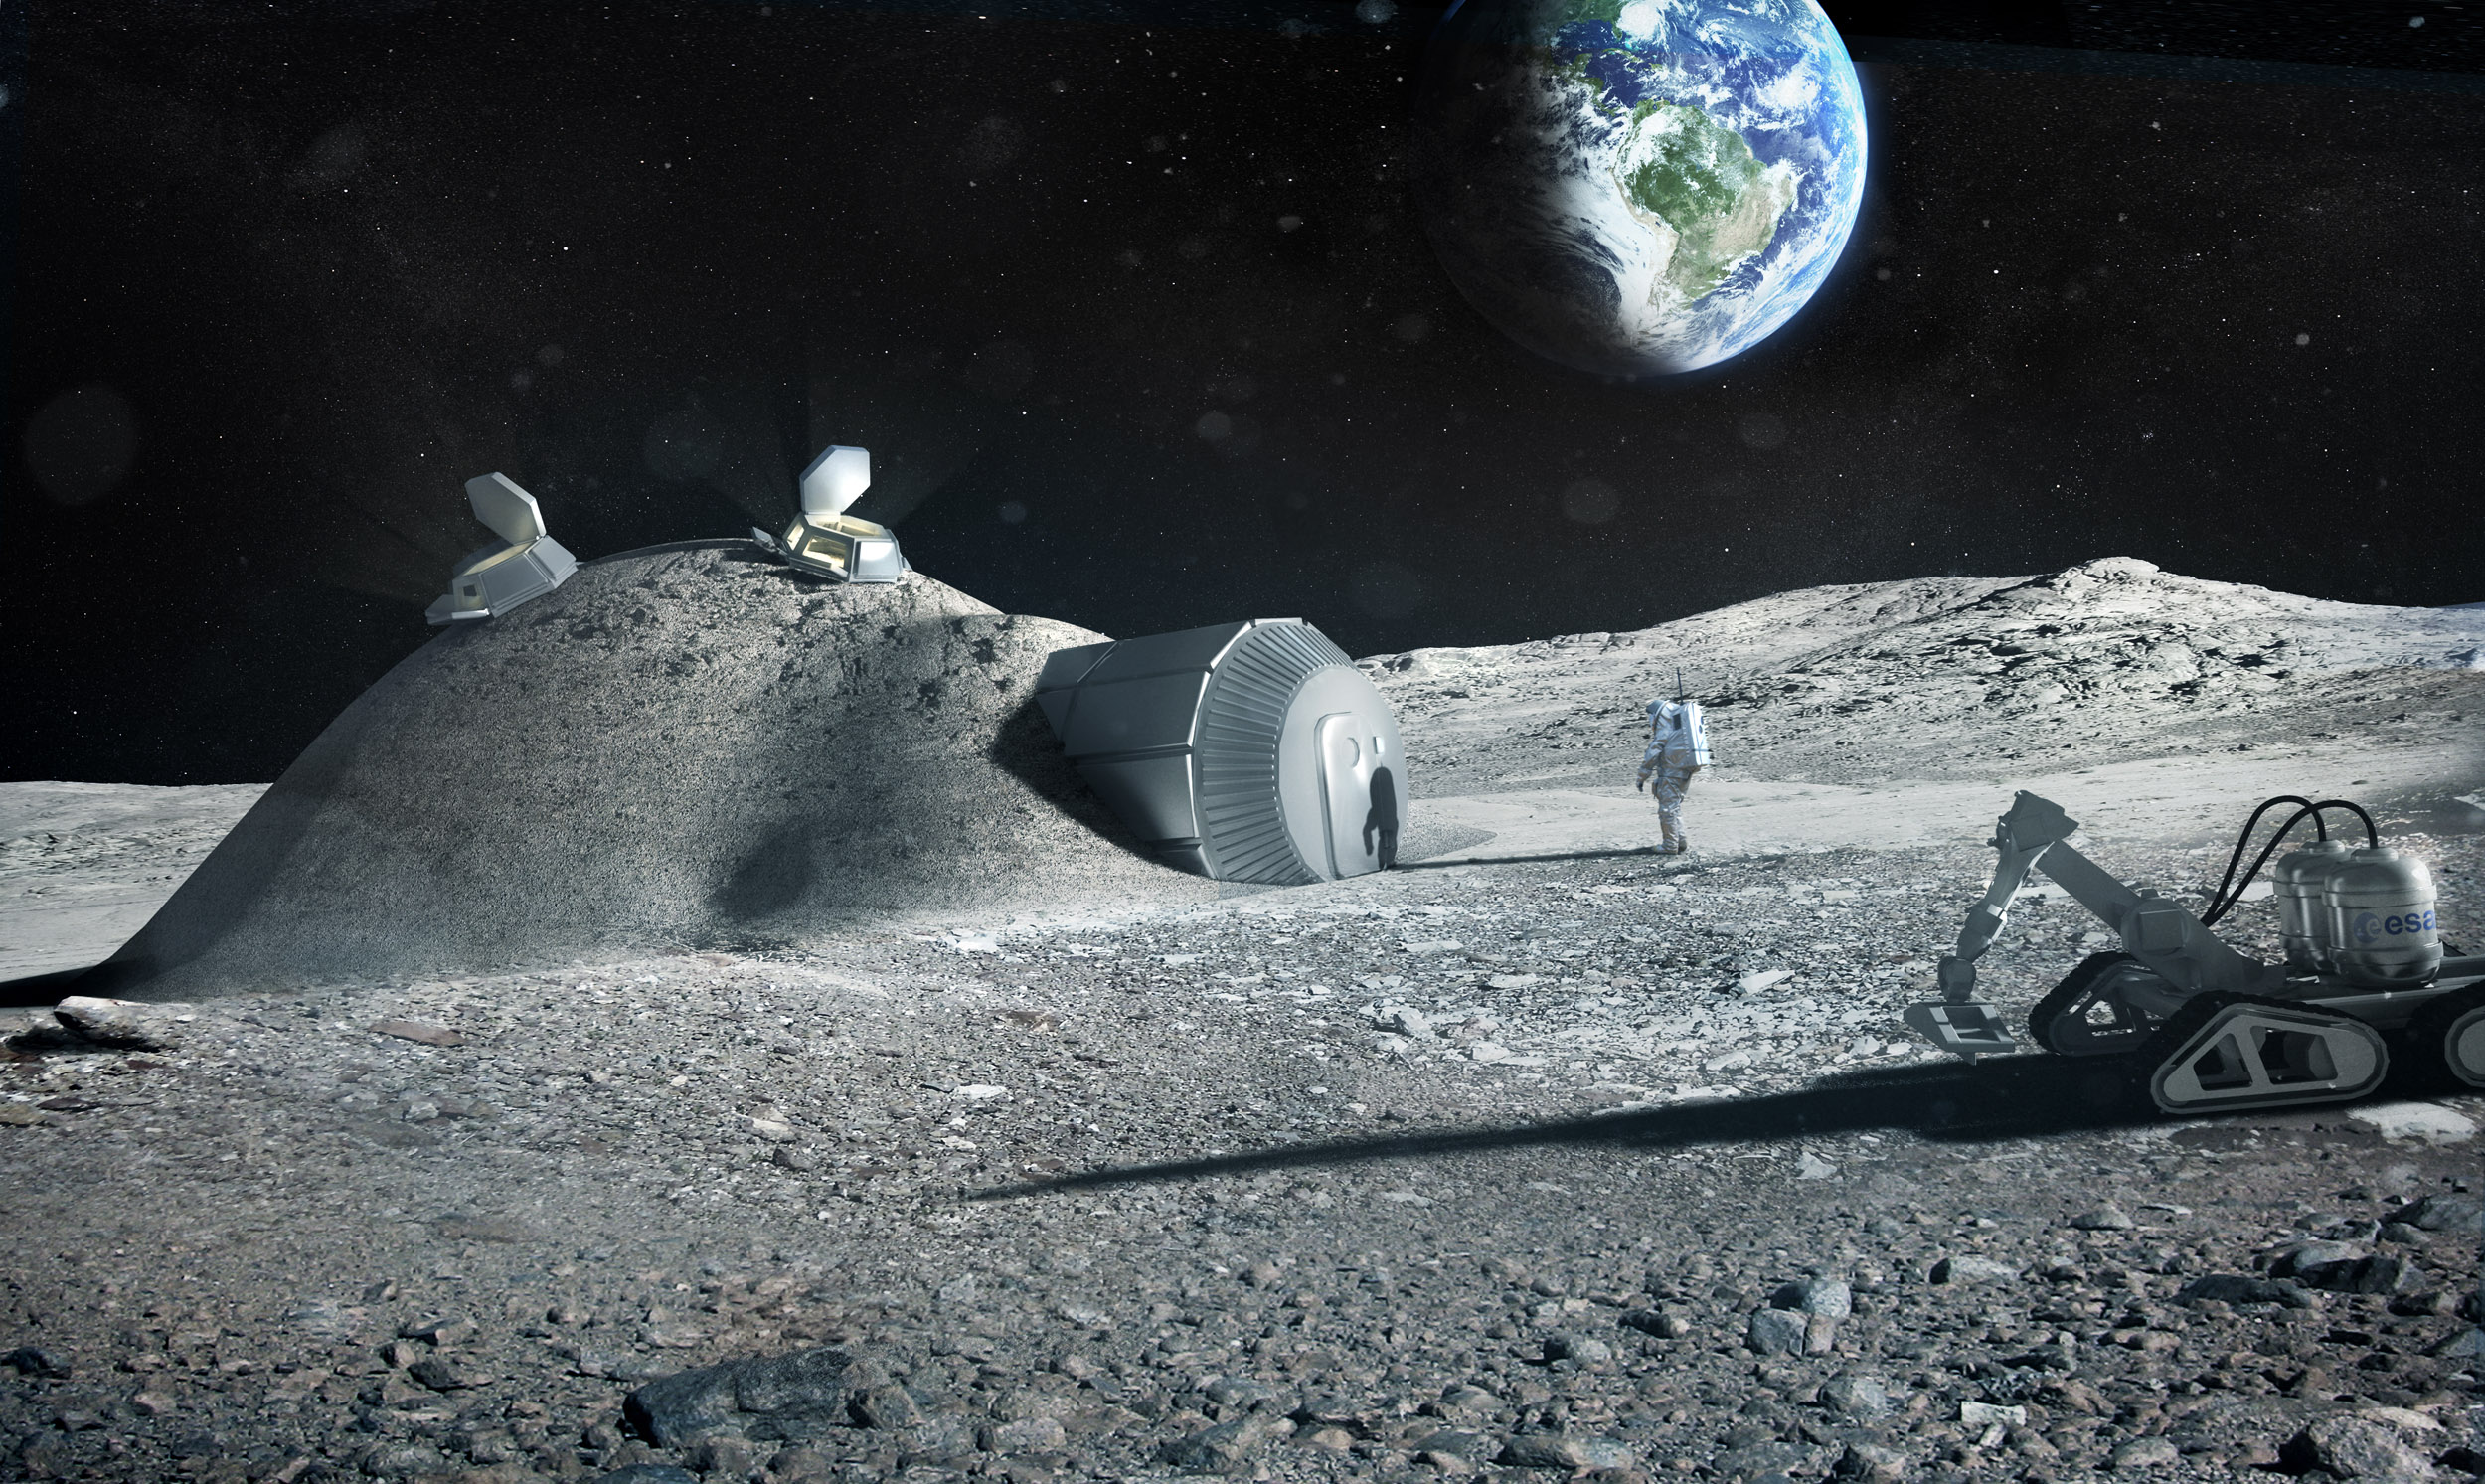
\includegraphics[height = 5cm]{../images/presentation/LunarBaseESA.jpg}
	   	\caption{Quelle: http://www.esa.int/spaceinimages/Images}
	\end{figure}
	
	%Lunar base aus 3D-Druck-Teilen und Mondgestein,
	%ESA (European Space Ageny)-Projekt,
	%Eurobot 2017-Wettbewerb unter diesem Moto

\end{frame} 

\begin{frame}
	\frametitle{Projektteam}
	
	\begin{figure}
		\begin{tikzpicture}[scale=0.5, transform shape]
		%Joel
		\def\xPos{2};	\def\yPos{1};
		\draw [draw=none, fill=hsrBlue] (\xPos - 2,\yPos - 4) rectangle (\xPos + 2,\yPos + 1);
		\draw [white] (\xPos,\yPos + 0.5) node{Joel Stolz};
		\draw [white] (\xPos,\yPos) node{\textbf{Mechanik}};
		\node[inner sep=0, outer sep=0, align=center] at (\xPos, \yPos - 2.2) {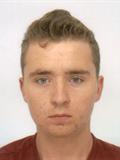
\includegraphics[height=3.5cm]{../images/Projektorganisation/joelStolz.jpg}};
		%Tibor
		\def\xPos{7};	\def\yPos{1};
		\draw [draw=none, fill=hsrBlue] (\xPos - 2,\yPos - 4) rectangle (\xPos + 2,\yPos + 1);
		\draw [white] (\xPos,\yPos + 0.5) node{Tibor Schneider};
		\draw [white] (\xPos,\yPos - 0) node{\textbf{Elektronik}};
		\node[inner sep=0, outer sep=0, align=center] at (\xPos, \yPos - 2.2) {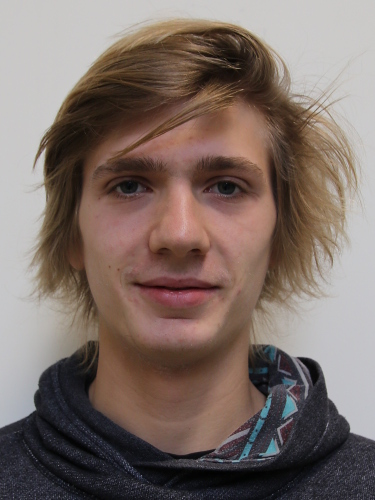
\includegraphics[height=3.5cm]{../images/Projektorganisation/tiborSchneider.jpg}};
		%cornel
		\def\xPos{12};	\def\yPos{1};
		\draw [draw=none, fill=hsrBlue] (\xPos - 2,\yPos - 4) rectangle (\xPos + 2,\yPos + 1);
		\draw [white] (\xPos,\yPos + 0.5) node{Cornel Angehrn};
		\draw [white] (\xPos,\yPos - 0) node{\textbf{Elektronik}};
		\node[inner sep=0, outer sep=0, align=center] at (\xPos, \yPos - 2.2) {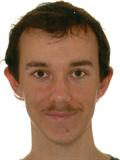
\includegraphics[height=3.5cm]{../images/Projektorganisation/cornelAngehrn.jpg}};
		%Matthias
		\def\xPos{17};	\def\yPos{1};
		\draw [draw=none, fill=hsrBlue] (\xPos - 2,\yPos - 4) rectangle (\xPos + 2,\yPos + 1);
		\draw [white] (\xPos,\yPos + 0.5) node{Matthias Knöpfel};
		\draw [white] (\xPos,\yPos - 0) node{\textbf{Elektronik}};
		\node[inner sep=0, outer sep=0, align=center] at (\xPos, \yPos - 2.2) {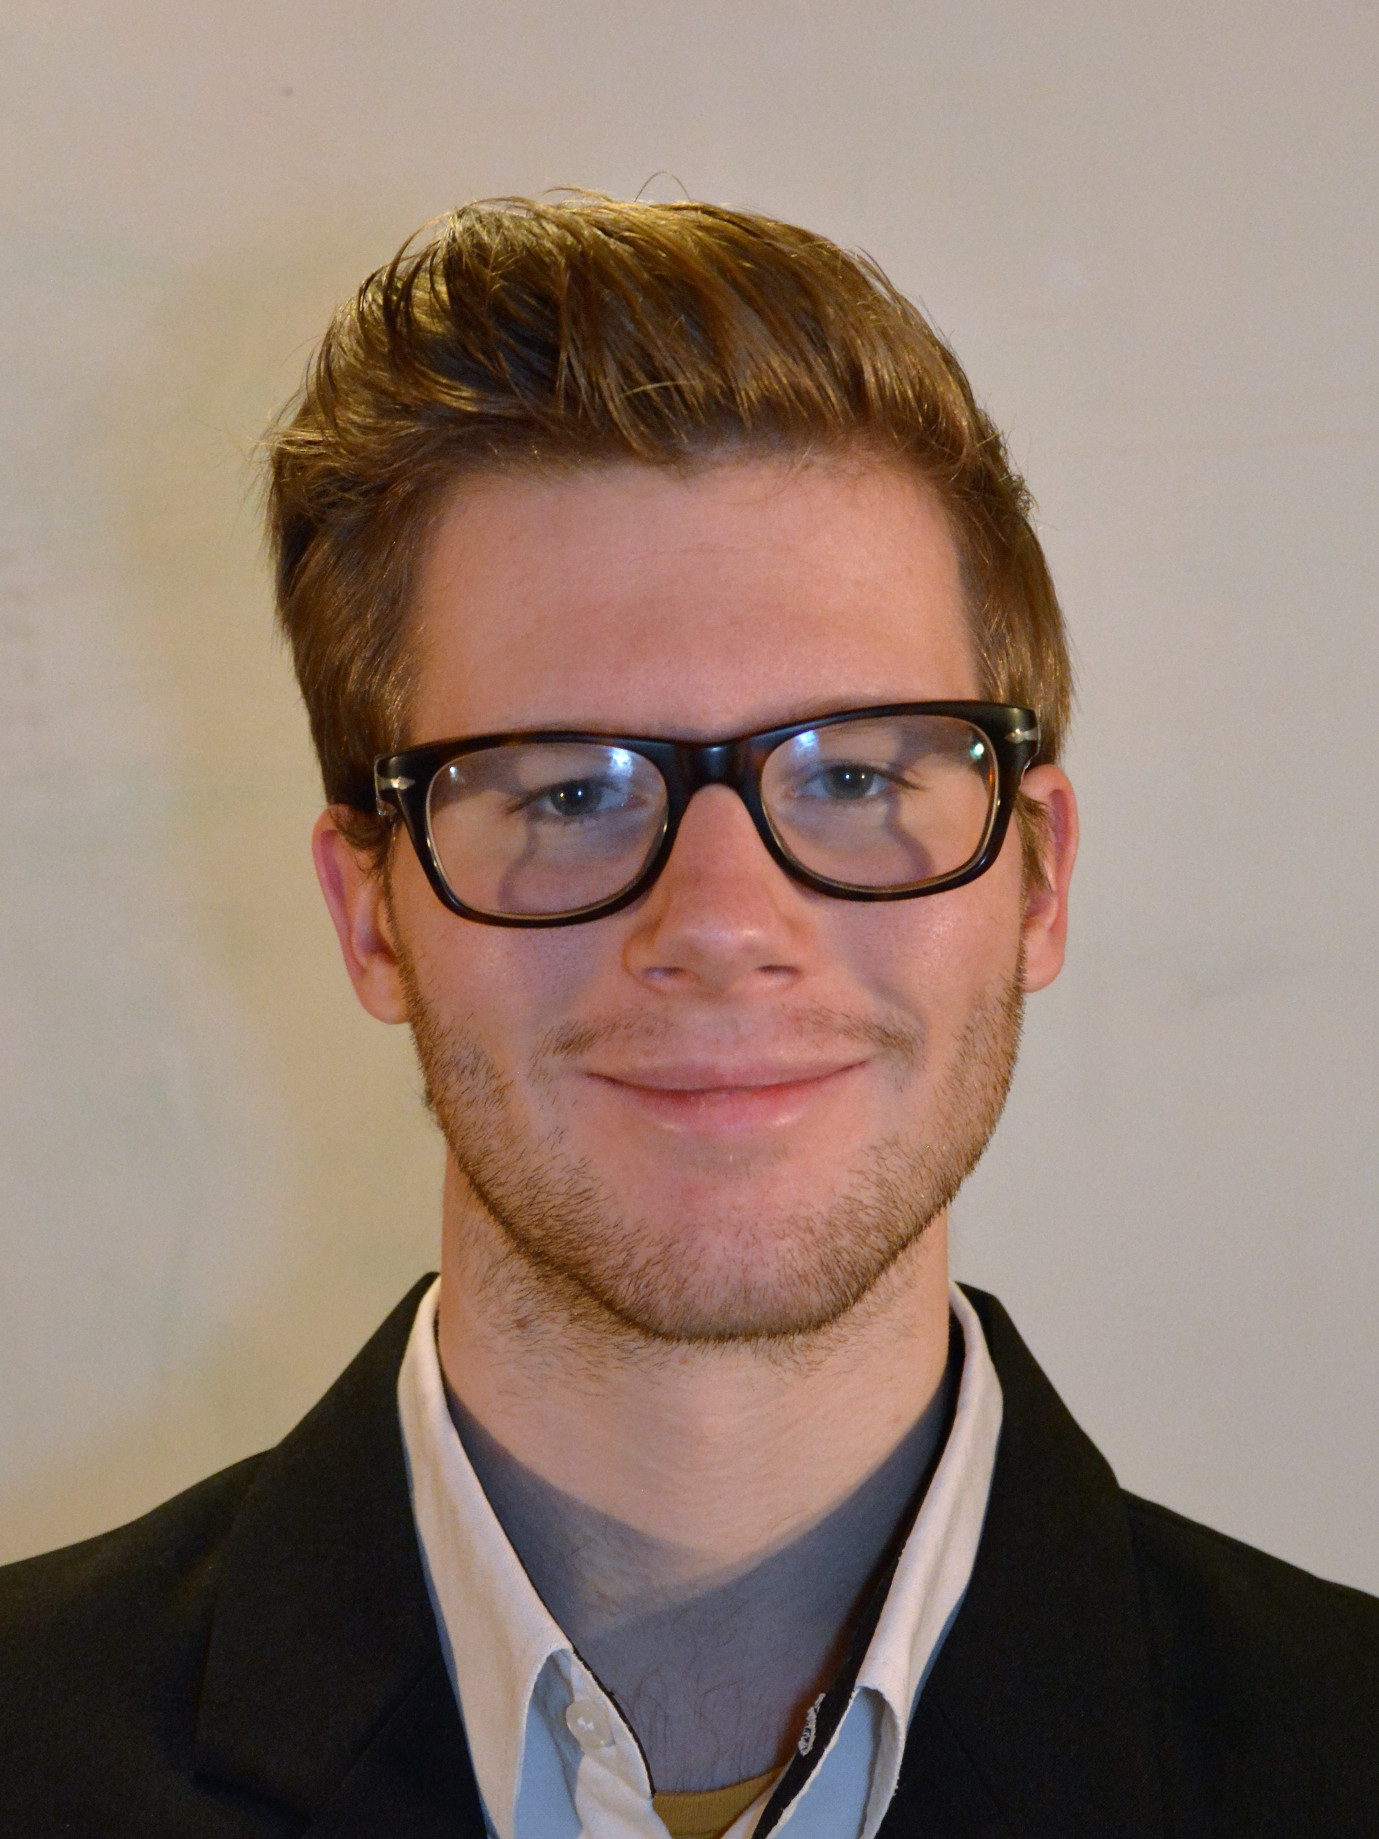
\includegraphics[height=3.5cm]{../images/Projektorganisation/matthiasKnoepfel.jpg}};
		%Petra
		\def\xPos{22};	\def\yPos{5};
		\draw [draw=none, fill=hsrBlue] (\xPos - 2,\yPos - 4) rectangle (\xPos + 2,\yPos + 1);
		\draw [white] (\xPos,\yPos + 0.5) node{Petra Freuler};
		\draw [white] (\xPos,\yPos - 0) node{\textbf{Projektanalyse}};
		\node[inner sep=0, outer sep=0, align=center] at (\xPos, \yPos - 2.2) {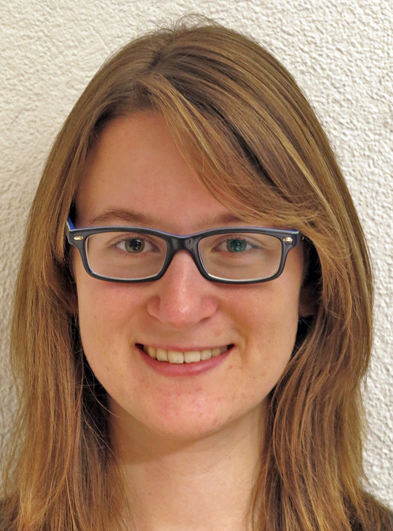
\includegraphics[height=3.5cm]{../images/Projektorganisation/petraFreuler.jpg}};
		%Wüst
		\def\xPos{2};	\def\yPos{8};
		\draw [draw=none, fill=hsrBlue] (\xPos - 2.5,\yPos - 1) rectangle (\xPos + 2.5,\yPos + 1);
		\draw [white] (\xPos,\yPos + 0.25) node{Prof. Theodor Wüst};
		\draw [white] (\xPos,\yPos - 0.25) node{\textbf{Betreuung Mechanik}};
		%Brändle
		\def\xPos{11};	\def\yPos{8};
		\draw [draw=none, fill=hsrBlue] (\xPos - 2.5,\yPos - 1) rectangle (\xPos + 2.5,\yPos + 1);
		\draw [white] (\xPos,\yPos + 0.5) node{Prof. Erwin Brändle};
		\draw [white] (\xPos,\yPos) node{\textbf{Auftraggeber}};
		\draw [white] (\xPos,\yPos - 0.5) node{\textbf{Betreuung Elektronik}};
		%Keller
		\def\xPos{17};	\def\yPos{8};
		\draw [draw=none, fill=hsrBlue] (\xPos - 2.5,\yPos - 1) rectangle (\xPos + 2.5,\yPos + 1);
		\draw [white] (\xPos,\yPos + 0.5) node{Prof. Daniel Keller};
		\draw [white] (\xPos,\yPos) node{\textbf{Betreuung}};
		\draw [white] (\xPos,\yPos - 0.5 ) node{\textbf{Projektanalyse}};
		
		%connections
		\draw [thick] (2,2) -- (2,7) (2,3) -- (17,3) (7,2) -- (7,3) (12,2) -- (12,3) (17,2) -- (17,3) (11,3) -- (11,5) -- (20,5) (11,5) -- (11,7) (16,5) -- (17,5) -- (17,7);
		\end{tikzpicture}
	\end{figure}

\end{frame}

\begin{frame}
	\frametitle{Arbeitsaufteilung}
	Bereits während der Studienarbeit erledigt:
	\begin{itemize}
		\item Konzepte erstellt
		\item Gegnererkennung, Fahrcontroller und Softwareteile Mainboard vorbereitet
	\end{itemize}
	\vspace{1em}
	Aufgaben Bachelorarbeit:
	\begin{itemize}
	   	\item Fertigstellung der elektrischen Komponenten
	   	\item Strategie-Einheit, Wegfindung, \textit{collision handling}
	   	\item Zusammenbau und Test
	\end{itemize}

\end{frame}